% !TeX root = index.tex
\iffalse
This chapter looks specifically at your results.
* You measured some samples. 
What values did you measure? 
Present them in a table or graph? 
How did you test whether they were good measurements? 
Were you looking to improve something? 
Are your new samples better than the old ones?

* You built a device; 
what tests did you run to make sure that it is running correctly?

* You calculated something or developed a new theory about something. 
How do you know how well it predicts? 
What tests did you run? 
What comparisons with the literature did you make?
* You coded or simulated something. 
What tests did you run to be sure it was working correctly? 

Describe what you want the reader to notice in the results. 
Give the facts, then give your analysis of the facts.
Present your graphs, figures, tables, photos, and equations needed to show what you accomplished.
Label everything clearly, using the recommendations given below in “Things to Look For”
\fi

\subsection{FPGA logic component composition}
This subsection looks at test and its results to find how much FPGA logic components each processor takes and what is composition of each part.

Test was performed with Quartus synthesis tool and viewing flow summary report. This report includes synthesised design metrics including total logic elements, registers, memory bits and other FPGA resources. Test will only look at logic elements and registers. Total number of logic elements was found out by synthesising full processors, then commenting relevant parts of code, re-synthesising and viewing changes in total logic elements. Such method may not be the most accurate, because during HDL synthesis circuit is optimised an unused connections removed. This means that more logic may be not synthesised than intended. 

There are four parts of each processor that will be tested: 
\begin{enumerate}
	\item \textbf{Common} - processor auxiliary logic that is used by both processors. It includes communication block with UART, RAM and PLL (Phase-Locked Loop, for master clock generation). 
	\item \textbf{ALU} - as described in section \ref{subsec:alu}, both processors have slightly different implementation of ALU.
	\item \textbf{Memory} - processors memory management, including stack.
	\item \textbf{Other} - reminding logic of processor that was not analysed.
\end{enumerate}

\begin{colfigure}
	\centering
	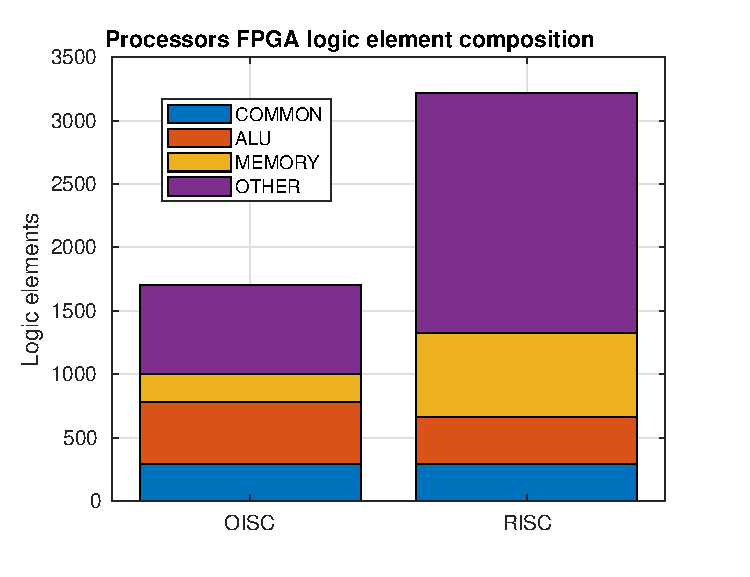
\includegraphics[width=\linewidth]{../tests/fpga_comp.eps}
	\captionof{figure}{Bar graph of FPGA logic components taken by each processor.}
	\label{fig:fpga_comp}
\end{colfigure}

Results of a test are shown in figures \ref{fig:fpga_comp} and \ref{fig:fpga_reg_comp}. Common logic uses 293 logic elements and 170 registers. OISC uses 1705 logic elements, while RISC uses 3218. Excluding common logic, OISC takes 48.3\% of RISC's logic elements.


\begin{colfigure}
	\centering
	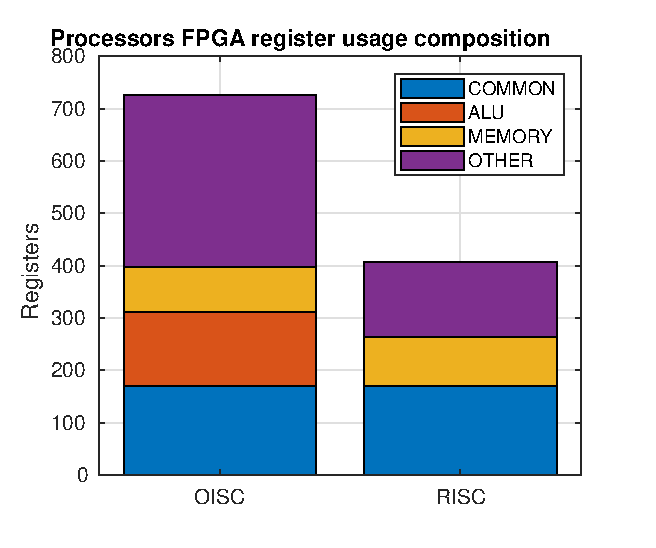
\includegraphics[width=\linewidth]{../tests/fpga_reg_comp.eps}
	\captionof{figure}{Bar graph of FPGA register resources taken by each processor.}
	\label{fig:fpga_reg_comp}
\end{colfigure}

OISC uses 726 logic elements, while RISC uses 407. Excluding common logic, OISC uses 78.4\% more registers than RISC.

Looking at composition, OISC ALU takes 30.2\% more logic gates. Looking at figure \ref{fig:fpga_reg_comp}, high number of OISC ALU registers can be observed which concludes, that higher resource usage is OISC ALU code include buffer logic.

Memory logic elements composition of OISC is only 34.4\% of RISC's and 7\% lower for register resources, comparing to RISC. This indicate that by removing memory logic for RISC, synthesis tool may removed also other parts of processor, possibly part of control block because it mostly contains combinational logic.

Other logic includes instruction decoding with ROM, register file, program counter. RISC exclusively has control block. Note that OISC uses  only three ROM memory blocks whereas RISC uses four as explained in section \ref{subsec:memory}, however this should make a minimal difference as M9K memory blocks are not included in FPGA logic element or register count. Comparing both processors, OISC has only 37\% of other logic components to RISC, however it has 2.28 times more registers. This shows a logic component - register trade-off. OISC buffer and common registers logic that connects bus require many more registers whereas RISC uses combination logic in control block in order to control same data in datapath. 

Much higher logic components in RISC can be also explained more complicated register file, ROM memory logic and program counter. All of these components has some additional logic for timing correction or additional functionality required by these blocks integration into datapath.

\subsection{Power analysis}

Power analysis was performed to analyse power consumption of both processors.
This has been accomplished by connecting FPGA board to a laboratory power supply with 4V to an external power input. A shunt resistor of was used of 1.020$\Omega$ was connected in series to calculate current. Supply voltage and voltage across shut resistor were measured using oscilloscope with data sampling feature. Multiple tests have been performed with different processor configurations. Between each tests a period of about 5 minutes was given for FPGA to reach steady state. 


\begin{colfigure}
	\centering
	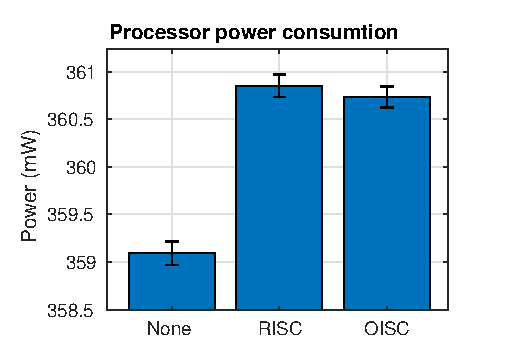
\includegraphics[width=\linewidth]{../tests/power.eps}
	\captionof{figure}{Measured power of processors when implemented on FPGA, running 16bit multiplication function in loop. None indicates auxiliary-only power.}
	\label{fig:power}
\end{colfigure}

Figure \ref{fig:power} represents power results. Auxiliary power includes whole FPGA board, voltage regulators, and synthesised logic on FPGA required to support a processor (such as PLL, UART, Input/Output control, RAM). RISC and OISC bars in the graph indicate auxiliary power plus processor power, which means that the processor itself takes relatively small amount comparing to auxiliary power, about 0.5\%.

During this test clock frequency of 1MHz was used. Due to equipment unavailability, further tests were not carried out to investigate power consumption at different frequencies. 

\subsubsection{Activity Factor}
An activity factor could be also found using Equation \ref{eq:activity_factor} where $P$ is power, $C_{total}$ indicate total gate capacitance and $V_{DD}$ indicate voltage supplied to the transistors.
\begin{align}\label{eq:activity_factor}
\alpha = \frac{P}{C_{total}\cdot f \cdot V_{DD}^2}
\end{align}
As $C_{total}$ and $V_{DD}$ are constants, measuring power at different frequencies allows finding activity factor. This value could be used to compare how much of a processor circuit is active. Further design improvements could be used to optimise power \autocite{8682289,7363689,1207041,6972455}.


\subsection{Benchmark Programs}
A number of and programs have been written to test both processors. These involve simple functions that could be commonly used in 8bit processors:

\begin{description}
	\item[$\bullet$ Printing:] Sends data to UART. It includes waiting until UART is available for transmission. 
	\item[$\bullet$ Printing unsinged integer:] Uses binary-coded decimal algorithm to convert 8 or 16bit binary value to decimal value and print it. 
	\item[$\bullet$ 16bit multiplication:] Uses simple matrix multiplication. 
	\item[$\bullet$ 16bit division:] Uses Long division algorithm to divide two 16bit numbers, result including a reminder.
	\item[$\bullet$ 16bit modulo:] Uses "Russian Peasant Multiplication" algorithm to perform Modulo operation with two 16bit numbers.
	\item[$\bullet$ Prime number calculator:] Uses Sieve of Atkins algorithm to calculate primer number, operates on 16bit numbers and utilise 16bit multiplication and modulo functions. 
\end{description}


\subsubsection{Instruction composition}\label{subsec:instr_comp}

This test is performed to investigate instruction composition of each function to see how similar it is between RISC and OISC processors. 
\begin{description}
	\item[$\bullet$ MOVE] - All instructions that move data around internal processor registers.
	\item[$\bullet$ ALU] - Instructions that are used to perform ALU operation.
	\item[$\bullet$ MEMORY] - Instructions that are required to send/retrieve data from system memory, except stack.
	\item[$\bullet$ STACK] - Instructions that push/pop data from memory stack.
	\item[$\bullet$ COM] - Instruction(s) that send/receive data from communication block.
	\item[$\bullet$ BRANCH] - Instructions that are used to make program branching.
	\item[$\bullet$ OTHER] - Any other instructions.
\end{description}

\begin{blockpage}
	\arrayrulecolor{black}
	\begin{tabular}{| c | p{0.65\linewidth} |} \hline 
		\rowcolor[rgb]{0.82,0.82,0.82}
		Name & Instructions \\\hline
		MOVE & \texttt{MOVE, CPY0, CPY1, CPY2, CPY3, CI0, CI1, CI2} \\\hline
		ALU & \texttt{%
			ADD, ADDI,
			SUB, SUBI,
			AND, ANDI,
			OR, ORI,
			XOR, XORI,
			DIV, MUL,
			ADDC, SUBC,
			INC, DEC,
			SLL, SRL, 
			SRA, GETAH
		} \\\hline
		MEMORY & \texttt{LWLO, LWHI, SWLO, SWHI} \\\hline
		STACK  & \texttt{PUSH, POP} \\\hline
		COM & \texttt{COM} \\\hline
		BRANCH & \texttt{BEQ, BGT, BGE, BZ, JUMP, CALL, RET} \\\hline
		\arrayrulecolor[rgb]{0,0,0}\hline
	\end{tabular}
	\captionof{table}{RISC processor instruction groups used in instruction composition test.}
	\label{tab:instr_groups_risc}
\end{blockpage}

\begin{blockpage}
	\arrayrulecolor{black}
	\begin{tabular}{| c | p{0.65\linewidth}|} \hline 
		\rowcolor[rgb]{0.82,0.82,0.82}
		Name & Destination \\\hline
		\arrayrulecolor[rgb]{0.82,0.82,0.82}
		MOVE & \texttt{REG0, REG1} \\\hline
		ALU & \texttt{ALU0, ALU1} \\\hline
		MEMORY & \texttt{MEM0, MEM1, MEM2, MEMLO, MEMHI} \\\hline
		STACK  & \texttt{STACK}\\\hline
		COM & \texttt{COMA, COMD}\\\hline
		BRANCH & \texttt{BR0, BR1, BRZ}\\\hline
		\arrayrulecolor[rgb]{0,0,0}\hline
	\end{tabular}
	\captionof{table}{OISC processor instruction desination groups used in instruction composition test}
	\label{tab:instr_groups_oisc_dst}
\end{blockpage}

\begin{blockpage}
	\arrayrulecolor{black}
	\begin{tabular}{| c | p{0.65\linewidth} |} \hline 
		\rowcolor[rgb]{0.82,0.82,0.82}
		Name & Instructions \\\hline	
		\arrayrulecolor[rgb]{0.82,0.82,0.82}	
		MOVE & \texttt{ALU0, ALU1, REG0, REG1, PC0, PC1, NULL, IMMEDIATE} \\\hline
		ALU & \texttt{ADD, ADDC, SUB, SUBC,
		AND, OR, XOR, SLL,
		SRL, EQ, GT, GE, NE,
		LT, LE, MULLO, MULHI, DIV, MOD,
		ADC, SBC, ROL, ROR} \\\hline
		MEMORY & \texttt{MEM0, MEM1, MEM2, MEMLO, MEMHI} \\\hline
		STACK  & \texttt{STACK} \\\hline
		COM & \texttt{COMA, COMD} \\\hline
		BRANCH & \texttt{BR0, BR1} \\\hline
		\arrayrulecolor[rgb]{0,0,0}\hline
	\end{tabular}
	\captionof{table}{OISC processor instruction source groups used in instruction composition test}
	\label{tab:instr_groups_oisc_src}
\end{blockpage}

Each function was ran on simulated processor, program counter and instruction been recorded into file at every cycle. File recording was done with SytemVerilog test bench, it started recording when program counter matched \texttt{.start} location and stopped when it matched \texttt{.done} location. Code shown in listings \ref{asmrisctest} and \ref{asm_oisc_test} enabled both location to be static, not depending on test function executed.

\begin{blockpage}
	\begin{lstlisting}[frame=single, caption={RISC assembly frame for executring tests}, emph={setup,start,done} label=asmrisctest]
	setup:
	JUMP .start
	.done:
	JUMP .done
	.start:
	; Setup values
	; Call function
	JUMP .done
	\end{lstlisting}
\end{blockpage}

\begin{figure*}[ht!]
	\centering
	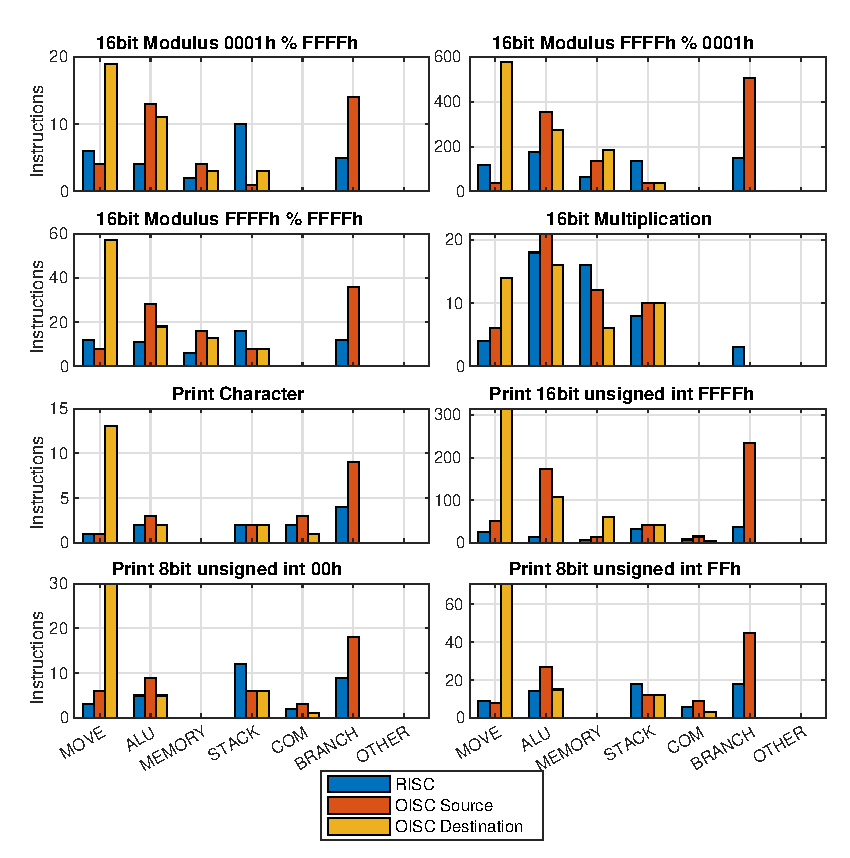
\includegraphics[width=\linewidth]{../tests/instr_comp.eps}
	\caption{Graph of instruction composition for every benchmark program.}
	\label{fig:instr_comp}
\end{figure*}

\begin{blockpage}
	\begin{lstlisting}[frame=single, caption={OISC assembly frame for executring tests}, emph={setup,start,done} label=asm_oisc_test]
	setup:
	BR1 .start @1
	BR0 .start @0
	BRZ 0x00
	.done:
	BRZ 0x00
	.start:
	; Setup values
	; Call function
	BR1 .done @1
	BR0 .done @0
	BRZ 0x00
	\end{lstlisting}
\end{blockpage}

Each function recorded file then was further analysed and each instruction was grouped. Recorded program counter was used to find effective program space. This has been achieved by calculating unique instances of program counter and summing up instruction size for each of them. In RISC, dynamic instruction size has been taken into account. 

From results in Figure \ref{fig:instr_comp} few key differences can be seen. Across every test, OISC has much more \textit{BRANCH} destination and \textit{MOVE} source groups. \textit{BRANCH} group can be explained by emulated \texttt{CALL}, \texttt{RET} and \texttt{JUMP} instruction explained in section \ref{subsec:oisc_pc}.
High number of \textit{MOVE} source group instructions may be explained by using immediate values as separate source, where RISC uses instruction that integrate with immediate in instructions such as \texttt{ADDI}. In most cases \textit{ALU} group instructions are also higher than for OISC comparing to RISC. This shows lower OISC ALU efficiency, mostly due to need to move data to septate accumulators.

\subsubsection{Performance}
This subsection investigates time and clock cycles to run benchmark programs. Simulation was sued to find a number of cycles required to execute each function. Note that prime number calculator was not simulated due to too complex dynamic nature of program. 

Print 16bit decimal and modulo operation were executed with different arguments to show the worst and the best case scenarios as algorithms length depend on inputs. This is not the case for 16bit multiplication as this it has no branching. 

Results are shown in Figure \ref{fig:cycles}. In most cases, OISC requires around 55-67\% more instruction, with some exceptions. These results can be better explained in following subsection \ref{subsec:instr_comp}.

\begin{colfigure}
	\centering
	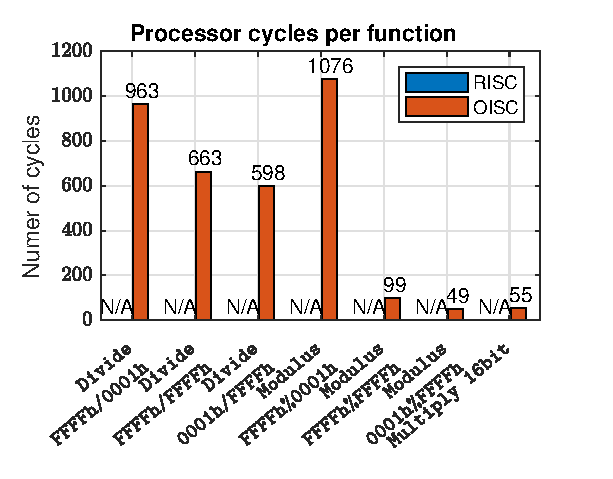
\includegraphics[width=\linewidth]{../tests/cycles.eps}
	\captionof{figure}{Simulated results of cycles that taken to perform function.}
	\label{fig:cycles}
\end{colfigure}

Another set of benchmarks have been performed and on both processors once they been implemented on FPGA. Time taken for perform each set has been recorded. This have been done via UART connection, a single character was sent to indicate start and stop of benchmark. In order to void slight timing variation due low baud rate of UART, each benchmark was performed many iterations. Figure \ref{fig:timing} represents results.

\begin{colfigure}
	\centering
	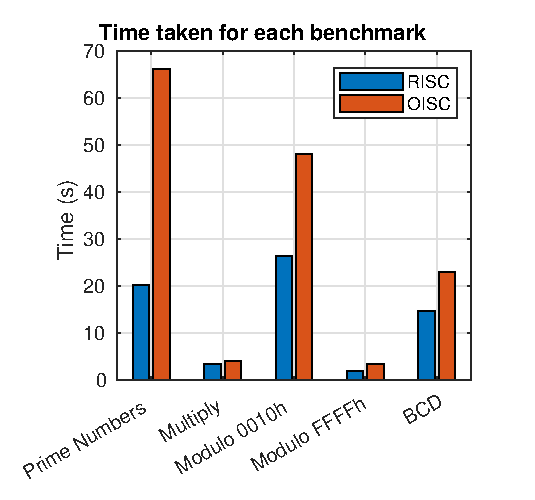
\includegraphics[width=\linewidth]{../tests/timing.eps}
	\captionof{figure}{Time taken perform each benchmark on FPGA.}
	\label{fig:timing}
\end{colfigure}

Results indicate that on average OISC takes about 71\% longer to execute same benchmark. This is close to results found with simulation. Prime number calculator have taken 3.26 times longer.

Benchmarks include:
\begin{description}
	\item[$\bullet$ Prime Numbers:] Calculate every prime number between 5 to $2^{16}$.  
	\item[$\bullet$ Multipy:] 16bit multiplication iterated 65536 times.
	\item[$\bullet$ Modulo 0010h:] 16bit \textit{0010h} modulo that operated on every number between 0 and 65536.
	\item[$\bullet$ Modulo FFFFh:] 16bit \textit{FFFFh} modulo that operated on every number between 0 and 65536.
	\item[$\bullet$ BDC:] Encoded 16bit binary to ASCII decimal number without printing.
\end{description}


\subsubsection{Program space}

Figure \ref{fig:program_size} represents effective program size for each test function. Effective program size only includes instruction that been executed depending on argument, meaning that it does not fully represent complete function. A specific argument might cause branching and skipping some function code which would not be added to effective program size. In this test, the main objective is to look difference in instruction size required to execute the same function, therefore not representing full program size is not relevant. 
\begin{colfigure}
	\centering
	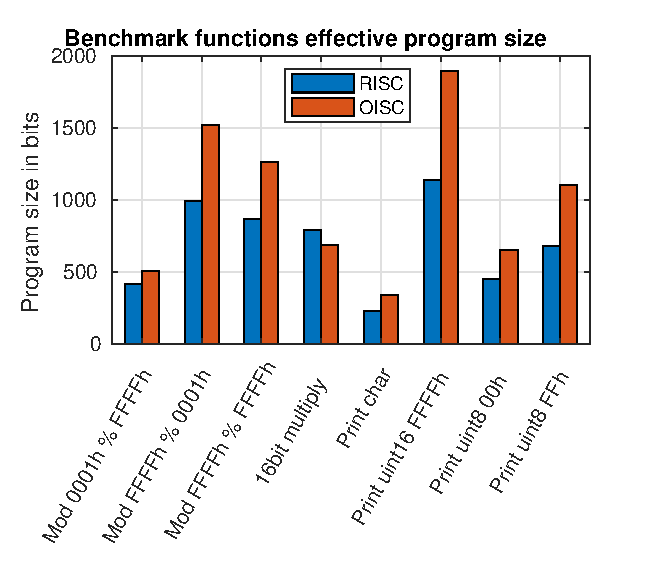
\includegraphics[width=\linewidth]{../tests/program_size.eps}
	\captionof{figure}{Bar graph showing effective size in bits each benchmark function is taking in program memeory.}
	\label{fig:program_size}
\end{colfigure}




\subsection{Maximum clock frequency}
To find maximum clock frequency, processors were loaded with basic print string function an d 16bit multiplication. Then frequency was constantly increased until resulting output though UART was not correct. 

In order to change clock frequency, three parameters were changed and HDL code resynthesised: 
\begin{description}
	\item[$\bullet$ PLL frequency multiplier and divider:]
	PLL takes 50MHz clock that is sourced from crystal on FPGA board and converts it to master clock $f_{mclk}$. Multiplier and divider values are used to adjust $f_{mclk}$.
	
	\item[$\bullet$ UART frequency divider:]
	Division value was calculated as $D = \left \lfloor \frac{f_{mclk}}{4 f_{baud}} \right \rfloor$. UART rate was set to 9600 baud. UART module itself has four times oversample. 
\end{description}
Frequency was changed in 5MHz increments. 

Theoretical maximum frequency was found using Quartus Timing Analysis tool. Slow 1200mV 85$^{\circ}$C model was used. 

\begin{center}
	\begin{tabular}{ l | c | c  }
		     & Theoretical & Actual \\ \hline
		RISC & 114.08MHz & 75-70MHz \\ \hline
		OISC & 64.68MHz & 45-40MHz \\
	\end{tabular}
	\captionof{table}{Theoretical and actual maximum frequencies of both processors.}
	\label{tab:max_freq}
\end{center}

Theoretical and actual results show unexpected results shown in Table \ref{tab:max_freq}, RISC operated at about 40\% higher maximum frequency than OISC.

As explained in Subsection \ref{subsec:oisc_cell_issue}, OISC logic blocks has about twice less time for data propagation. Keeping that in mind, and assuming that latch propagation and register setup periods are insignificant to critical path of OISC logic block, maximum OISC frequency could be double as high as, reaching 80-90MHz. This also assumes that there is no other part of processor would have limit. Further timing analysis needs to be carried out to confirm this.

\subsection{Future work}
\colorbox{yellow}{Description to be added.}

